% Gemini theme
% https://github.com/anishathalye/gemini

\documentclass[final]{beamer}

% Compile with lualatex.

% ====================
% Poster
% ====================

\usepackage[size=A0, orientation=portrait]{beamerposter}
\usetheme{gemini}
\usecolortheme{mit} %Modified...

% ====================
% Packages
% ====================

\usepackage[super]{cite}
\usepackage[super,sort&compress]{natbib}
\usepackage{atbegshi}
\usepackage{booktabs}

% ====================
% Font
% ====================

\usepackage[utf8]{inputenc}
\usepackage[T1]{fontenc}
\usepackage[usefilenames,DefaultFeatures={Ligatures=Common}]{plex-otf} %
\renewcommand*\familydefault{\sfdefault} %% Only if the base font of the document is to be sans serif
%\usepackage{lmodern}

\renewcommand{\baselinestretch}{1.1}

% ====================
% Graphics
% ====================

\usepackage{graphicx}
\usepackage{pgfplots}

\usepackage{color}
\usepackage{xcolor}
    \definecolor{ver00}{HTML}{18974C}   % EMBL green            ┐
    \definecolor{ver01}{HTML}{0A5032}   % Darkest tint green    │
    \definecolor{ver02}{HTML}{007B53}   % Dark tint green       ├ EMBL primary colours
    \definecolor{ver03}{HTML}{6CC24A}   % Light tint green      │
    \definecolor{ver04}{HTML}{D0DEBB}   % Lightest tint green   ┘
    \definecolor{gre00}{HTML}{707372}   % EMBL grey             ┐
    \definecolor{gre01}{HTML}{373A36}   % Darkest tint grey     │
    \definecolor{gre02}{HTML}{54585A}   % Dark tint grey        ├ EMBL secondary neutral colours
    \definecolor{gre03}{HTML}{A8A99E}   % Light tint grey       │
    \definecolor{gre04}{HTML}{D0D0CE}   % Lightest tint grey    ┘
    \definecolor{red00}{HTML}{D41645}   % EMBL red
    \definecolor{ora00}{HTML}{F49E17}   % EMBL orange
    \definecolor{ebi_petrol}{HTML}{389196}	% EBI Petrol	    ┐
    \definecolor{ebi_blue}{HTML}{008CB5}	% EBI Blue	    │
    \definecolor{ebi_green}{HTML}{9fcc3b}	% EBI Green	    ├ EBI Colours
    \definecolor{ebi_yellow}{HTML}{e6b222}	% EBI Yellow	    │
    \definecolor{ebi_grey}{HTML}{c3c0ab}	% EBI Grey	    ┘

\usepackage{tikz}
\usetikzlibrary{calc}
\usetikzlibrary{matrix}
\usetikzlibrary{positioning}
\usetikzlibrary{shapes.geometric, shapes.arrows, arrows}
\tikzstyle{feature} = [rectangle, minimum width=0.8\columnwidth, minimum height=2cm, text centered, draw=ver00, fill=ver00, text=white]
\tikzstyle{sub_feature} = [rectangle, minimum width=0.4\columnwidth, minimum height=1.5cm, text centered, draw=ebi_blue, fill=ebi_blue, text=white]
\tikzstyle{ftp_feature} = [rectangle, minimum width=0.4\columnwidth, minimum height=1.5cm, text centered, draw=ora00, fill=ora00, text=white]
\tikzstyle{exp_feature} = [rectangle, minimum width=0.8\columnwidth, minimum height=2cm, text centered, draw=ebi_yellow, fill=ebi_yellow, text=white]
\tikzstyle{dash_arr} = [dashed,ultra thick,->,>=stealth,red00]
\tikzstyle{cont_arr} = [ultra thick,->,>=stealth,red00]

% ====================
% Lengths + Pos
% ====================

\usepackage[absolute,overlay]{textpos}
  \setlength{\TPHorizModule}{1mm}
  \setlength{\TPVertModule}{1mm}

% If you have N columns, choose \sepwidth and \colwidth such that
% (N+1)*\sepwidth + N*\colwidth = \paperwidth
\newlength{\sepwidth}
\newlength{\colwidth}
\setlength{\sepwidth}{0.025\paperwidth}
\setlength{\colwidth}{0.4625\paperwidth}

\newcommand{\separatorcolumn}{\begin{column}{\sepwidth}\end{column}}

% ====================
% Title
% ====================

\title{\textcolor{mitred}{Ensembl Rapid Release 2022}}
\author{Jose Perez-Silva, Carlos Garcia-Giron, Thibaut Hourlier, Denye Ogeh, \\William Stark, Francesca Tricomi, Leanne Haggerty, Fergal Martin}
\institute[shortinst]{\inst{} Genebuild Team, Ensembl, EMBL-EBI, Hinxton, UK.}

% ====================
% Footer
% ====================

\footercontent{
  \begin{columns}[t]
  \separatorcolumn
  \begin{column}{0.3\paperwidth}
  %\vspace{0.5\baselineskip}
  \textcolor{mitred}{}\\
  \textcolor{mitred}{ ereboperezsilva@ebi.ac.uk}
  \\
  \end{column}
  \separatorcolumn
  \begin{column}{0.3\paperwidth}
  
  \end{column}
  \separatorcolumn
  \begin{column}{0.3\paperwidth}
    \rightline{EMBL’s European Bioinformatics Institute (EMBL-EBI)}
    \rightline{Wellcome Genome Campus, Hinxton. CB10 1SD. UK.}
    \rightline{T +44(0)1223 494 444}
  \end{column}
  \separatorcolumn
  \end{columns}
}


% ====================
% Body
% ====================

\begin{document}

\begin{textblock}{20}(20,23)
    \sloppy
    
\includegraphics[scale=1]{figures/ensembl-logo}
\end{textblock}

\begin{textblock}{20}(655,23)
    \sloppy
    
\includegraphics[scale=0.57]{figures/embl-ebi}
\end{textblock}

% ====================
% first column
% ====================

\begin{frame}[t]

\begin{columns}[t]
\separatorcolumn
\begin{column}{\colwidth}

\begin{block}{Introduction}

As we see the biodiversity of our planet diminish in the midst of a “sixth extinction event” fuelled by human activities, an international \textit{call to action} has been issued to preserve, store and analyse the genetic richness of Nature.
In response, a number of global sequencing projects have arisen, with the goal to sequence all life on the planet.
Examples include the Darwin Tree of Life project, which aims to sequence the genomes of 70,000 species of eukaryotic organisms in Britain and Ireland and the Vertebrate Genome Project, aiming to complete reference genomes for around 70,000 vertebrates.

Similarly, a continuous improvement, availability and affordability of sequencing and assembly technologies have made it possible to answer the \textit{call to action} quickly and efficiently all over the world, with lots of teams actively working on acquiring samples, sequencing species and assembling genomes to the highest quality ever.

As a result, we have seen an increase in high quality genome submissions and annotation requests, having currently around a hundred of genome submissions monthly, being a large percentage of it from non-vertebrates.
In order to support this new influx of genomes we have need to adapt both our annotation system and the release method.

\begin{figure}
  \centering
  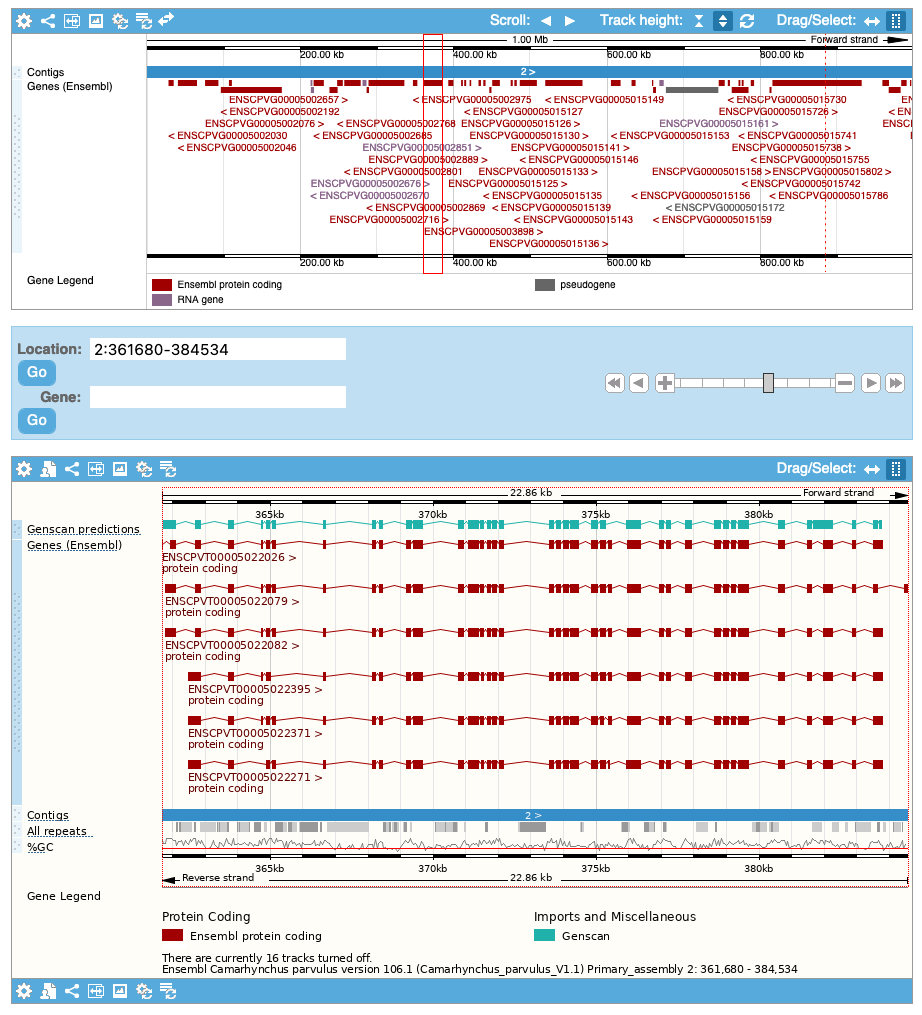
\includegraphics[width=0.95\columnwidth]{eg.png}      
    \caption{Screenshot of the genome browser for a especific genomic region in the Rapid Release website. Much like the main Release site, we can see the chosen genomic region, gene predictions in the selected range, repeats detected, percentage of Cs and Gs, and supporting matherial among others. The displayed channels can be edited as usual, and every predicted gene or element can be selected for more info or direct access to it.}
  \label{tree}
\end{figure}

In recent years we have massively scaled our automatic annotation pipelines, and we are now capable of annotating many species in a very short time.
This means that we are able to deliver annotation data at a faster rate and we require a platform for this, one that is not tied to a three-month cycle.
The new Ensembl website, which allow for more dynamic integration of data, is currently in development, so in the meantime we have created an intermediate solution – the Rapid Release.

The \textbf{Ensembl Rapid Release} is a lightweight genome browser, updated on a two week cycle, and designed to be more responsive than the main Ensembl website.
There we can upload the results of our annotation efforts more frequently, hence providing a much quicker answer to the consortium's needs.
Although Ensembl Rapid Release is not as fully featured as a typical data release on ensembl.org, for each species, we do provide a gene set along with additional features such as protein feature annotation, BLAST functionality, homologous relationships with an appropriate set of reference species and HAL multiple alignments for selected clades.

\end{block}

\begin{block}{Other features}

We recently included homology predictions for all available annotated genomes.
To make this predictions we use the software Diamond, which identifies the closes homologue between the queried genome and a set of representatives.
These sets include vertebrata, mammalia, actinopterigii, sauropsida, hexapoda, and a generic group for genomes that won't fit in the previous cathegories.
The generic set is an extension of this core group.
More representatives are under development.
Additionally, we present some multiple alignment (HAL) for different batches of Lepidoptera.

We are currently working on providing variation data.

\end{block}

%\vspace{}

\begin{figure}
    \centering
    \begin{tikzpicture}[align=center,rounded corners]
        \node (ank)[]{};
        \node (web)[draw, single arrow, shape border rotate=180, fill=ver00, minimum height=.29\colwidth, text centered, draw=ver00, text=white,above=of ank]{Ensembl\\Rapid Release};
        \node (ftp)[draw, single arrow, minimum height=.29\colwidth, text centered, draw=ebi_blue, fill=ebi_blue,text=white,below=of ank]{Rapid Release\\FTP Site};
        \node (qrrr)[inner sep=10pt,left=5cm of ank]{
\includegraphics[scale=0.27]{qr}};
        \node (qrbi)[inner sep=10pt,right=5cm of ank]{
\includegraphics[scale=0.27]{qr}};
    \end{tikzpicture}
\end{figure}

% ====================
% Second column
% ====================

\end{column}

\separatorcolumn
\setbeamertemplate{caption}[default]

\begin{column}{\colwidth}

\begin{figure}
  \centering
  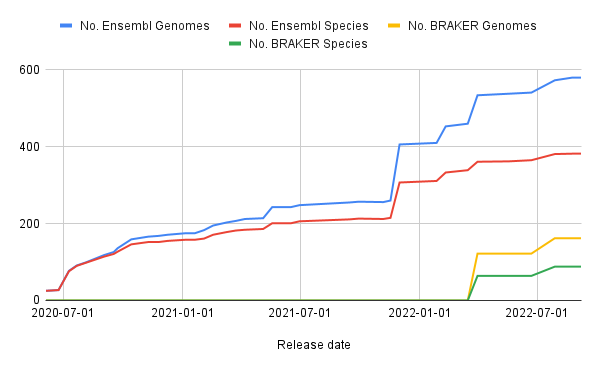
\includegraphics[width=0.9\columnwidth]{chart.png}
  \renewcommand{\thefigure}{2}
  \caption{This figure be more info.}
  \label{tree}
\end{figure}

\begin{block}{Features}

Currently, the site hosts over 500 non-vertebrate genomes (more than half of whcih are Lepidoptera assemblies, but also includes Diptera, Hymenoptera, Coleoptera, and even Mollusca).
Additionally to the assemblies analysed by Ensembl, the site includes a browser for external annotations that we have imported due to interest from the community.
Some examples of this include non-vertebrate species for which communities have a vested interest, including insects, worms, and even plants

We have adapted our long-standing annotation-system and tuned to work better for non vertebrates annotations.
This tailored adaptation includes methods to allow accurate determination of protein coding genes in the absence of sufficiently informative data from the projection and homology pipeline.
Althought it lacks some of the functionalities our vertebrate pipeline has, it is still in development and we are investigating new software and methods to annotate specific gene types, such as miRNAs, Ig, pseudogenes, lncRNAs, and more.

While many species have (or will soon have) transcriptomic data available, there is a large and rapidly growing number of high-quality genome assemblies that do not have suitable transcriptomic data.
Despite this absece of supporting evidence for the annotation, we recognised a desire by the communities to have acces to a draft genome.
To tackle this we we have started to run BRAKER2, to generate hint-guided ab initio gene predictions of protein-coding genes, using clade-specific proteins from UniProt and OrthoDB to run in the default protein mode.
This annotation will be distincly marked by the tag "BRAKER" in the "Annotation method" field.

\begin{figure}
    \centering
    \begin{tikzpicture}[align=center,rounded corners]
        \node (f1)[feature]{Annotated Geneset};
        \node (f1a)[sub_feature,below=of f1.south east, anchor=north east]{Stable IDs};
        \node (f1b)[sub_feature,below=of f1a]{Splice variants};
        \draw [cont_arr] (f1.195) |- (f1a.180);
        \draw [cont_arr] (f1.195) |- (f1b.180);
        \node (f2)[feature,below=of f1b.south east,anchor=north east]{Repeats annotation};
        \node (f2a)[ftp_feature,below=of f2.south east, anchor=north east]{Softmasked genome};
        \draw [cont_arr] (f2.195) |- (f2a.180);
        \node (f3)[feature,below=of f2a.south east,anchor=north east]{BLAST tool};
        \node (f3a)[sub_feature,below=of f3.south east, anchor=north east]{BLASTN};
        \node (f3b)[sub_feature,below=of f3.south east, anchor=north east]{TBLASTX};
        \draw [cont_arr] (f3.195) |- (f3a.180);
        \draw [cont_arr] (f3.195) |- (f3b.180);
        \node (f4)[feature,below=of f3b.south east,anchor=north east]{File dumps};
        \node (f4a)[ftp_feature,below=of f4.south east,anchor=north east]{Protein sequences};
        \node (f4b)[ftp_feature,below=of f4a.south east,anchor=north east]{Transcript sequences};
        \draw [cont_arr] (f4.195) |- (f4a.180);
        \draw [cont_arr] (f4.195) |- (f4b.180);
        \node (f5)[feature,below=of f4b.south east,anchor=north east]{Compative genomics};
        \node (f5a)[sub_feature,below=of f5.south east,anchor=north east]{Homology prediction};
        \node (f5b)[ftp_feature,below=of f5a.south east,anchor=north east]{Multiple alignments};
        \draw [cont_arr] (f5.195) |- (f5a.180);
        \draw [cont_arr] (f5.195) |- (f5b.180);
        \node (f6)[exp_feature,below=of f5b.south east,anchor=north east]{Variation info};
    \end{tikzpicture}
    \caption{Detailed list of the features that can be found in the Rapid Release Website. \textcolor{ora00}{Orange} features can be downloaded from the FTP site, the \textcolor{ebi_blue}{blue} ones can be found in the browser. \textcolor{ebi_yellow}{Yellow} features are in development.}
\end{figure}

As per today, Ensembl Rapid Release website hosts around 900 different genomes from some 600 species.
Of these, a vast majority belong to the Insecta taxa, with a large percentage of them being part of the DToL project. 

\end{block}

\begin{block}{Acknowledments}

The design and development of the Ensembl Rapid Release is a collective effort of the \textit{Ensembl Team}, part of the European Molecular Biology Laboratory's European Bioinformatics Institute (\textbf{EMBL-EBI}). 

\end{block}

\end{column}

\separatorcolumn

\end{columns}

\end{frame}

\newpage
\AtBeginShipout{%
\AtBeginShipoutDiscard
}
\bibliographystyle{nature}
\bibliography{poster}

\end{document}
